\section{BitsAboutMe}
BitsAboutMe ist ein in der Schweiz ansässiges Unternehmen, welches eine Plattform bereitstellt, auf der man seine Daten verwalten und gleichzeitig verkaufen kann.

\subsection{Ziel}
Als Ziel setzt sich das Unternehmen, den Nutzern mehr Kontrolle über die eigenen Daten zu geben. Damit soll ein fairer Datenhandel zwischen Datenkonsumenten und Datenanbietern geschaffen werden, sowie eine aktive Teilnahme an der Monetariserung dieser. Weiterhin lädt das Unternehmen jedoch auch weitere Unternehmen ein, an diesem Netzwerk teilzunehmen und bietet unterschiedliche Analysen und Auswertungsmöglichkeiten, sowie eine Schnittstelle zu den Datenanbietern.

\subsection{Rollen bei BitsAboutMe}
\textbf{Nutzer:} Nutzer können auf der Plattform, ähnlich wie im Abschnitt \ref{invisibly} bei Invisibly, ihre Daten von diversen Konten, wie Instagram, Facebook, Spotify, Amazon aber auch E-Mail- und Bankkonten hinzufügen. Neben dem Verkauf von persönlichen Daten soll ein Überblick über die Daten des Nutzers an einem zentralen Ort verschafft werden. Der Nutzer kann durch den Import verschiedener Datenquellen herausfinden, wie das eigene Nutzungsverhalten in sozialen Netzwerken ist, wie groß der eigene CO\textsubscript{2}-Fußabdruck ist oder ob man einen gesunden Lifestyle führt. Um damit nur einige Möglichkeiten zu nennen, hat der Nutzer also damit die Möglichkeit die Daten der jeweiligen Datenquellen einzusehen und aggregiert darzustellen und sich auswerten zu lassen. \newline

\noindent Der Nutzer fungiert demzufolge wiederum als Datenanbieter beziehungsweise Datenquelle, wobei jedoch die Privatsphäre im Vordergrund steht. BitsAboutMe garantiert durch eine Verschlüsselung der Datenbank auf Nutzerebene und einem Rechenzentrum in der EU oder in der Schweiz für eine hohe Sicherheit und ausschließliche Einsicht der Daten durch den Nutzer selbst. Dieser kann mithilfe der \gls{PWA} stets selbst entscheiden, welche Daten konkret freigegeben werden und welche nicht.\newline

\begin{figure}[!htbp]
	\centering
	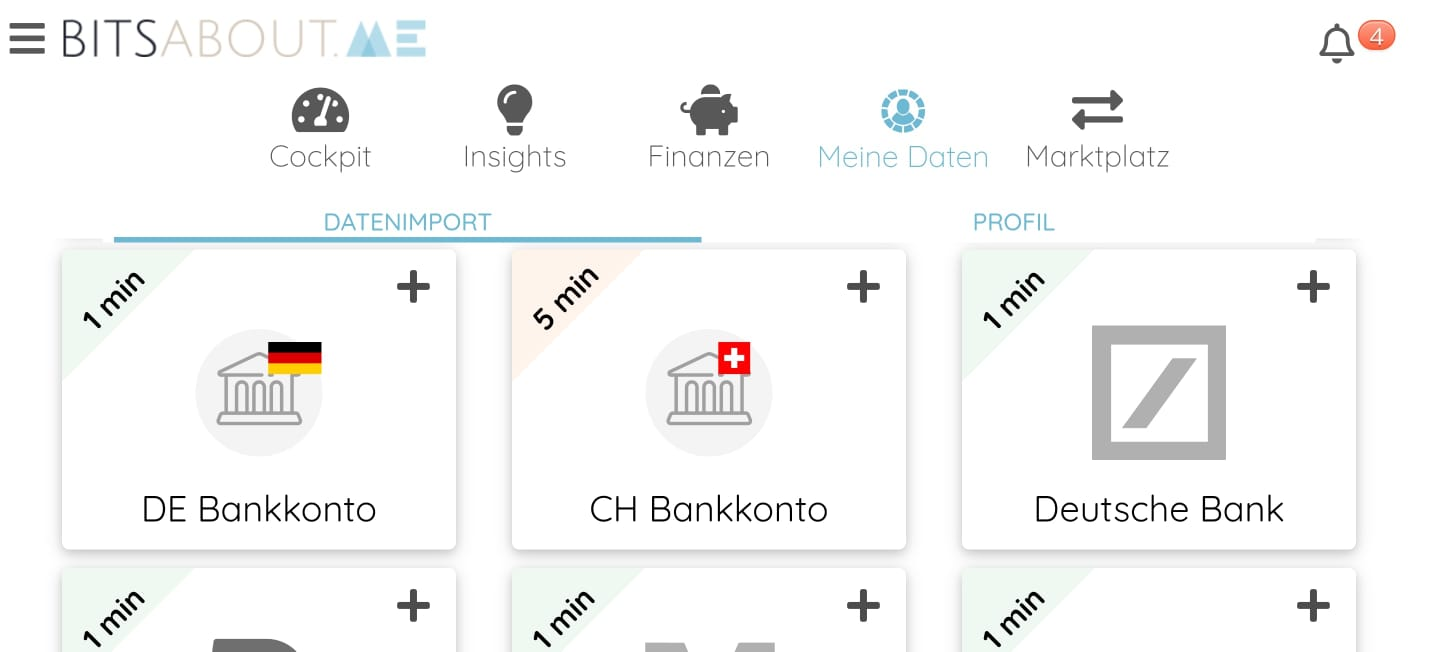
\includegraphics[width=\textwidth]{bitsaboutme_datenquellen}
	\caption{Möglichkeiten des Hinzufügens von Datenquellen auf der BitsAboutMe-Plattform mit ungefährer Zeitabschätzung}
	\label{fig:bitsaboutmeDatenquellen}
\end{figure}
\FloatBarrier

\noindent \textbf{Käufer:} Käufer auf der BitsAboutMe-Plattform sind Unternehmen, welchen BitsAboutMe eine SaaS-Lösung anbietet, mit der sie als Datenkonsumenten die bereitsgestellten Daten von Nutzern erwerben können und Überblick über stattgefundene Trankaktionen erhalten.

\subsection{Daten auf der BitsAboutMe-Plattform monetarisieren}
Damit der Nutzer die persönlichen Daten nun monetarisieren kann, bietet er eine Auswahl der Daten nun auf dem Daten-Marktplatz an. BitsAboutMe verfolgt dabei eine getrennte Architektur vom persönlichen Datenspeicher (im Folgenden \textit{PDS} genannt) und dem persönlichen Daten-Marktplatz (im Folgenden \textit{PDM} genannt). Das bedeutet, dass die Daten bei dem Verknüpfen der Konten mit der BitsAboutMe-Plattform vorerst verschlüsselt im PDS abgelegt werden, worauf der Nutzer alleinig zugreifen kann. Entschließt dieser sich nun zu einem Verkauf dieser, so werden diese anonymisiert und an den PDM transferiert, sodass durch den Nutzer ausgewählte Datenkonsumenten beziehungsweise Unternehmen Zugriff auf das Datenprofil haben. Durch das Teilen des Datenprofils verdient der Nutzer Geld. Zusätzlich erhält BitsAboutMe ebenfalls eine Gebühr für die Transaktion.\newline

\noindent Möchte der Nutzer jedoch zukünftig nicht mehr sein anonymisiertes Datenprofil zur Verfügung stellen, so ist eine Rücknahme oder eine Löschung des Datenprofils jederzeit möglich. \newline

\begin{figure}[h!]
	\centering
	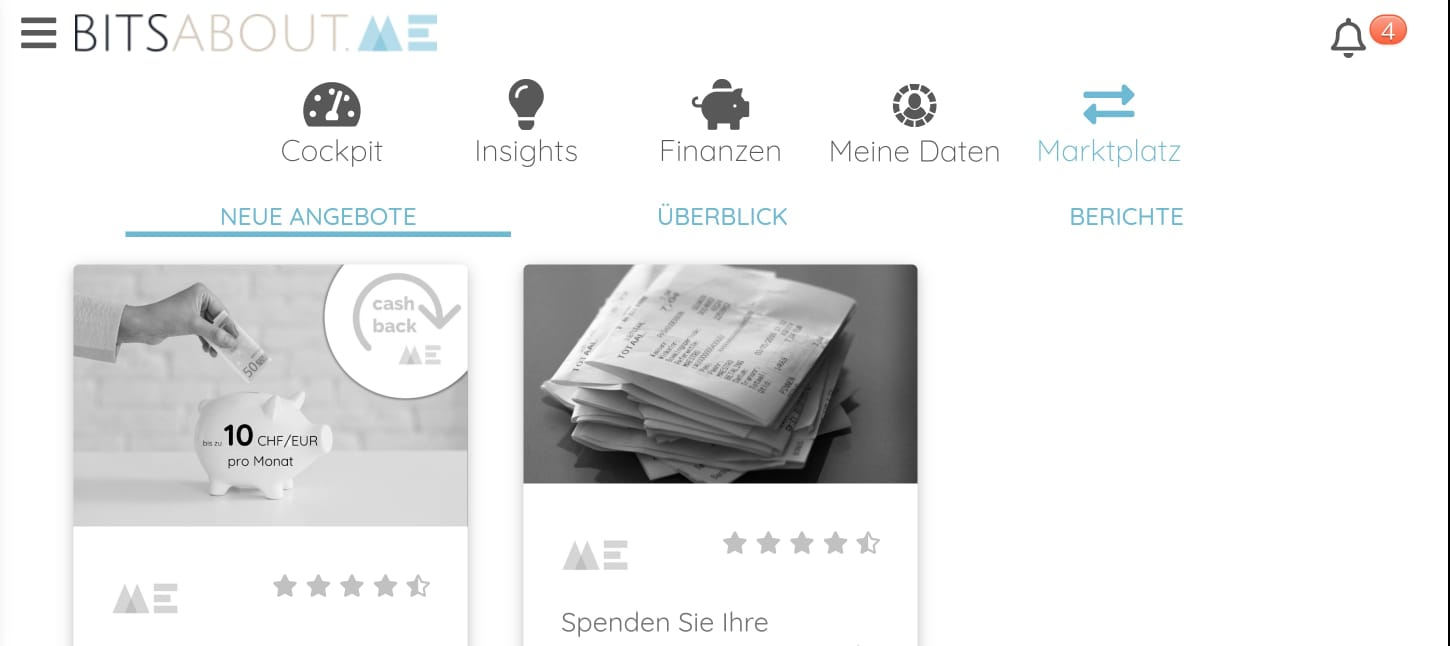
\includegraphics[width=\textwidth]{bitsaboutme_marktplatz.jpg}
	\caption{Persönlicher Datenmarktplatz auf der BitsAboutMe-Plattform mit Angeboten, angenommen Angeboten und Informationen zu abgerufenen Daten}
	\label{fig:bitsaboutmeMarktplatz}
\end{figure}
\FloatBarrier

\noindent Neben dem Teilen des Nutzerprofils bietet die Plattform noch eine weitere Möglichkeit Daten anonym zu monetarisieren. Undzwar kann der Nutzer von ihm erhaltene Kassenzettel einscannen und 1\% Cashback auf den jeweiligen Einkauf erhalten. Dies ist jedoch auf 10€ im Monat begrenzt. Diese Daten fließen ebenfalls in das persönliche Benutzerprofil ein, da BitsAboutMe anhand dessen analysiert, wie nachhaltig und gesund der Nutzer lebt und gleichzeitig einen Überblick über die Finanzen schafft. Damit die Daten valide sind und damit brauchbar für die Datenkonsumenten, werden die Kassenbons mit den Zahlungen des hinterlegten Bankkontos abgeglichen. Nur auf Zahlungen, die auf dem Bankkonto durchgeführt wurden, gibt es Cashback. Unternehmen können diese Daten folglich erwerben und für die Marktforschung und andere, im Abschnitt \ref{datenoekonomie} Datenökonomie, beschriebene Zwecke nutzen. \newline

\noindent Zusammengefasst sind folgende Schritte für die Monetariserung der Daten notwendig:
\begin{enumerate}
	\item Registieren
	\item Datenquellen verbinden
	\item (digitale Identität prüfen)
	\item PDM aktivieren
	\item Daten freigeben und Geschäft abschließen
\end{enumerate}
